\documentclass[ngerman,hyperref={pdfpagelabels=false}]{beamer}

% -----------------------------------------------------------------------------

\graphicspath{{images/}}

% -----------------------------------------------------------------------------

\usetheme{KIT}

\setbeamercovered{transparent}
%\setbeamertemplate{enumerate items}[ball]

\newenvironment<>{KITtestblock}[2][]
{\begin{KITcolblock}<#1>{#2}{KITblack15}{KITblack50}}
{\end{KITcolblock}}

\usepackage[ngerman,english]{babel}
\usepackage[utf8]{inputenc}
\usepackage[TS1,T1]{fontenc}
\usepackage{array}
\usepackage{multicol}
\usepackage[absolute,overlay]{textpos}
\usepackage{beamerKITdefs}
\usepackage{algorithmic}

\pdfpageattr {/Group << /S /Transparency /I true /CS /DeviceRGB>>}	%required to prevent color shifting withd transparent images


\title{Algorithmen I - Tutorium 3}
\subtitle{Sebastian Schmidt -- \textit{isibboi@gmail.com}}

\author[Sebastian Schmidt]{Sebastian Schmidt}
\institute{Arbeitsgruppe Kryptographie und Sicherheit}

\TitleImage[width=\titleimagewd,height=\titleimageht]{titel}

\KITinstitute{Arbeitsgruppe Kryptographie und Sicherheit}
\KITfaculty{Fakult\"at f\"ur Informatik}

% -----------------------------------------------------------------------------

\begin{document}
\setlength\textheight{7cm} %required for correct vertical alignment, if [t] is not used as documentclass parameter


% title frame
\begin{frame}
  \maketitle
\end{frame}


\begin{frame}{Folien}
Online unter: https://github.com/ISibboI/AlgoI-Tut
\end{frame}

\newcommand{\nat}{\mathbb{N}}

\begin{frame}
\footnotesize
    \begin{algorithmic}[1]
      \STATE \textbf{function} \textit{merge}($A : $ Array $[1..n_1]$ of $\nat_{\geq 0} $, $B : $ Array $[1..n_2]$ of $\nat_{\geq 0} $)
	\STATE \textbf{assert} $A[i] \leq A[j]$ \quad $ \forall i \leq j$ mit  $i, j \in \{1,..., n_1\}$
	\STATE \textbf{assert} $B[i] \leq B[j]$ \quad $ \forall i \leq j$ mit $i, j \in \{1,..., n_2\}$
	\STATE $A[n_1+1] := \infty$, $B[n_2+1] := \infty$
	\STATE $n := n_1 + n_2$ 
	\STATE $j_A := 1$, $j_B := 1$;
      	\STATE \textbf{for} $i:=1$ \textbf{to} $n$ \textbf{do}
        \STATE \quad $C[i] = \min(A[j_A],B[j_B])$
        \STATE \quad \textbf{if} $A[j_A] < B[j_B]$ \textbf{then}  	
        \STATE \quad \quad $j_A = j_A + 1$ 
	\STATE \quad \textbf{else}	
        \STATE \quad \quad $j_B = j_B + 1$ 
        \STATE \quad \textbf{invariant} $C[1..i]$ enthält genau $A[1..j_A-1], B[1..j_B-1]$ 
	\STATE \quad \textbf{invariant} $B[k] \leq A[j_A] \quad  \forall k \in \{1..j_B-1\}$, $A[k] \leq B[j_B]\quad  \forall k \in \{1..j_A-1\}$ 
	\STATE \quad \textbf{invariant} $C[1..i]$ ist sortiert 
        \STATE \textbf{assert} $j_A = n_1+1, j_B = n_2 + 1$ 
        \STATE \textbf{assert}  $C[i] \leq C[j]$ \quad $ \forall i \leq j,$ $i, j \in \{1,..., n\}$
        \STATE \textbf{assert} $C[1..n]$ enthält genau $A[1..n_1], B[1..n_2]$ 
      \RETURN C
    \end{algorithmic}
\end{frame}

\section{Übungsblatt}

\begin{frame}{Übungsblatt 1}
\begin{itemize}[<+->]
\item Aufgabe 1.a.3) Formal korrekt\linebreak
$n^2 \log n \in O\left(n^3\right)$
\item Aufgabe 1.c) Hatte niemand richtig\linebreak
$\forall f, g : \mathbb{N} \rightarrow \mathbb{N}: f(n) \in O(g(n)) \Rightarrow 2^{f(n)} \in O\left(2^{g(n)}\right)$
\end{itemize}
\end{frame}


\section{Wiederholung}

\begin{frame}{Wiederholung}
\begin{itemize}
\item<1-> Einfach verkettete Liste
\item<2-> Doppelt verkettete Liste
\item<3-> Unbounded Array
\item<4-> Unbounded queue mit doppelt verketteter Liste
\begin{itemize}
\item Direkt
\item Mit splice
\end{itemize}
\end{itemize}
\end{frame}

\begin{frame}{splice}
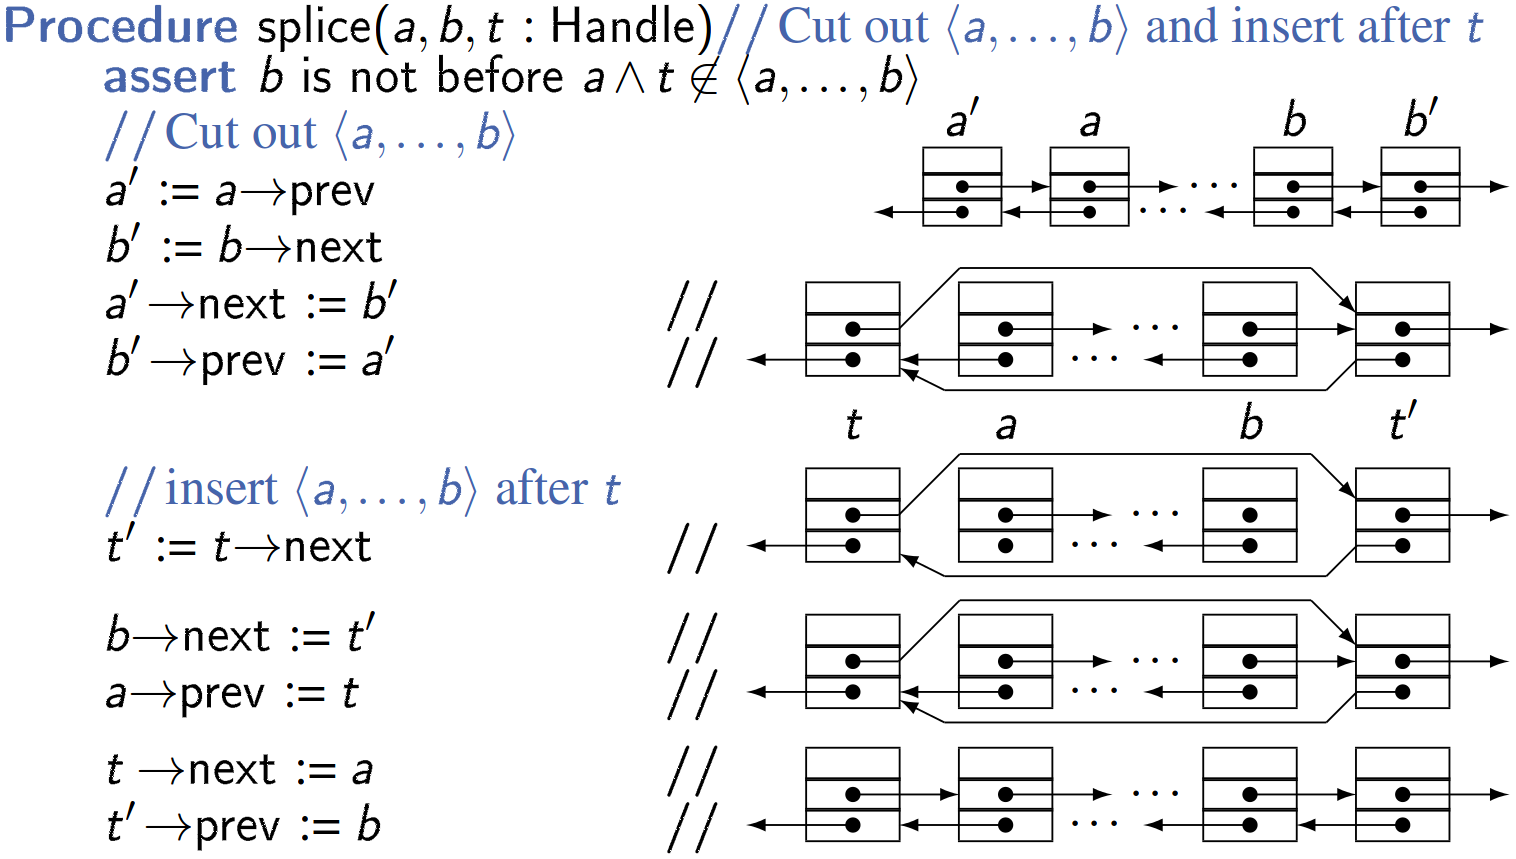
\includegraphics[width=\textwidth]{splice}
\end{frame}


\section{Aufgaben}

\begin{frame}{Aufgabe 1.a}
Entwickelt eine Datenstruktur, die folgendes kann:
\begin{itemize}
\item \texttt{pushBack} und \texttt{popBack} in $O(1)$ Zeit im Worst-Case
\item Wahlfreier Zugriff in $O(\log n)$ Zeit im Worst-Case
\end{itemize}

Nicht amortisiert!

Speicherallokation geht hier in konstanter Zeit.
\end{frame}

\begin{frame}{Aufgabe 1.b}
Entwickelt eine Datenstruktur, die folgendes kann:
\begin{itemize}
\item \texttt{pushBack} und \texttt{popBack} in $O(\log n)$ Zeit im Worst-Case
\item Wahlfreier Zugriff in $O(1)$ Zeit im Worst-Case
\end{itemize}

Nicht amortisiert!

Speicherallokation geht hier in konstanter Zeit.
\end{frame}

\begin{frame}{Aufgabe 2}
Was passiert, wenn man \texttt{splice(a, b, t : Handle)} fälschlicherweise mit $\texttt{t} \in \langle \texttt{a}, \dots, \texttt{b}\rangle$ aufruft?
\end{frame}

\begin{frame}{Aufgabe 3}
Gegeben ist ein Array $A = A[1], \dots, A[n]$ mit $n$ Zahlen in beliebiger Reihenfolge.

Suche für eine gegebene Zahl $x$ ein Paar $(A[i], A[j]), 1 \leq i, j, \leq n$ mit $A[i] + A[j] = x$.

\begin{itemize}
\only<1-2>{\item<1-> Beispiel: Gebt eine Lösung für $x = 33$ und $A = (7, 15, 21, 14, 18, 3, 9)$ an.
\item<2-> Gebt einen Algorithmus an, der das Problem in erwarteter Zeit $O(n)$ lößt, und bei Erfolg ein Paar $(A[i], A[j])$ ausgibt, ansonsten $NIL$.}
\only<3>{\item Sei $c \in \mathbb{N}$ fest.
\item Gebt einen Algorithmus an, der das Problem in deterministischer Zeit $O(n)$ für natürliche Zahlen $A[i] \leq c \cdot n$ lößt, und bei Erfolg ein Paar $(A[i], A[j])$ ausgibt, ansonsten $NIL$.}
\only<4>{\item Haben wir noch Zeit?
\item Gebt einen Algorithmus an, der das Problem in deterministischer Zeit $O(n)$ für Ganzzahlen lößt, und bei Erfolg ein Paar $(A[i], A[j])$ ausgibt, ansonsten $NIL$. Hinweise:
\begin{itemize}
\item Wir befinden uns im RAM-Modell mit fixer Wortbreite. Darin kann man ganze Zahlen in $O(n)$ sortieren.
\end{itemize}}
\end{itemize}
\end{frame}

\end{document}
